\begin{figure}[!ht]



\centering
\tikzset{every picture/.style={line width=0.75pt}} %set default line width to 0.75pt        

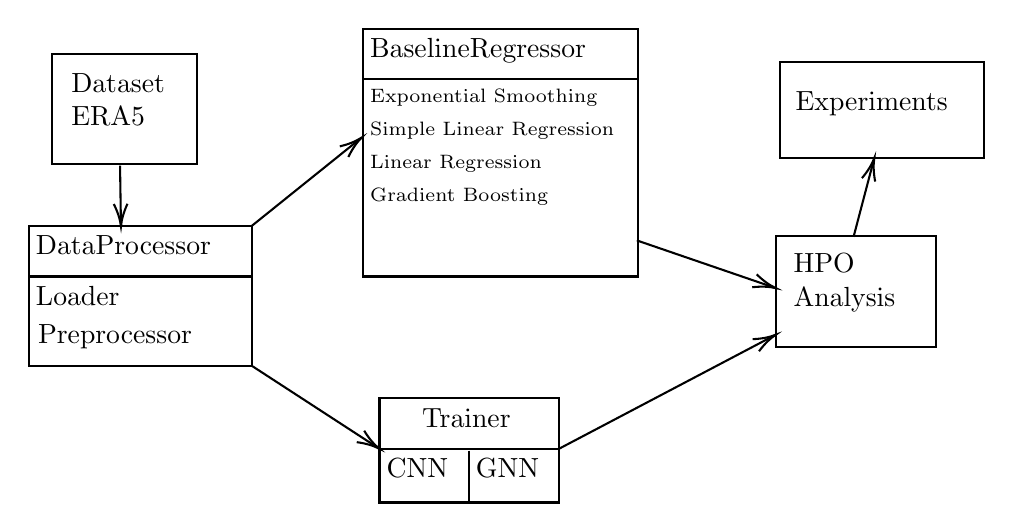
\begin{tikzpicture}[x=0.75pt,y=0.75pt,yscale=-1,xscale=1]
%uncomment if require: \path (0,300); %set diagram left start at 0, and has height of 300

%Shape: Rectangle [id:dp7530154494125894] 
\draw   (49,24) -- (119,24) -- (119,77.4) -- (49,77.4) -- cycle ;
%Shape: Rectangle [id:dp9698514264995771] 
\draw   (38,107) -- (145.47,107) -- (145.47,131.4) -- (38,131.4) -- cycle ;
%Shape: Rectangle [id:dp4969191214073878] 
\draw   (199,12) -- (331.47,12) -- (331.47,36.4) -- (199,36.4) -- cycle ;
%Shape: Rectangle [id:dp46276974315458586] 
\draw   (38,131.4) -- (145.47,131.4) -- (145.47,174.4) -- (38,174.4) -- cycle ;
%Shape: Rectangle [id:dp4183627533315526] 
\draw   (199,36.4) -- (331.47,36.4) -- (331.47,131.4) -- (199,131.4) -- cycle ;
%Straight Lines [id:da828734951299678] 
\draw    (82,78) -- (82.42,105.35) ;
\draw [shift={(82.45,107.35)}, rotate = 269.12] [color={rgb, 255:red, 0; green, 0; blue, 0 }  ][line width=0.75]    (10.93,-3.29) .. controls (6.95,-1.4) and (3.31,-0.3) .. (0,0) .. controls (3.31,0.3) and (6.95,1.4) .. (10.93,3.29)   ;
%Straight Lines [id:da875811037343577] 
\draw    (145.47,107) -- (196.91,65.65) ;
\draw [shift={(198.47,64.4)}, rotate = 141.21] [color={rgb, 255:red, 0; green, 0; blue, 0 }  ][line width=0.75]    (10.93,-3.29) .. controls (6.95,-1.4) and (3.31,-0.3) .. (0,0) .. controls (3.31,0.3) and (6.95,1.4) .. (10.93,3.29)   ;
%Shape: Rectangle [id:dp5982407723060675] 
\draw   (207,190) -- (293.47,190) -- (293.47,214.4) -- (207,214.4) -- cycle ;
%Shape: Rectangle [id:dp127024224882344] 
\draw   (207,214.4) -- (293.47,214.4) -- (293.47,240.27) -- (207,240.27) -- cycle ;
%Straight Lines [id:da4532096531120119] 
\draw    (250.23,215.33) -- (250.23,239.33) ;
%Straight Lines [id:da6114762439202708] 
\draw    (145.47,174.4) -- (205.32,213.31) ;
\draw [shift={(207,214.4)}, rotate = 213.03] [color={rgb, 255:red, 0; green, 0; blue, 0 }  ][line width=0.75]    (10.93,-3.29) .. controls (6.95,-1.4) and (3.31,-0.3) .. (0,0) .. controls (3.31,0.3) and (6.95,1.4) .. (10.93,3.29)   ;
%Shape: Rectangle [id:dp9581227071990494] 
\draw   (398,112) -- (475,112) -- (475,165.4) -- (398,165.4) -- cycle ;
%Straight Lines [id:da27282092476109177] 
\draw    (331,114) -- (396.11,136.35) ;
\draw [shift={(398,137)}, rotate = 198.95] [color={rgb, 255:red, 0; green, 0; blue, 0 }  ][line width=0.75]    (10.93,-3.29) .. controls (6.95,-1.4) and (3.31,-0.3) .. (0,0) .. controls (3.31,0.3) and (6.95,1.4) .. (10.93,3.29)   ;
%Straight Lines [id:da6527635281271343] 
\draw    (293.47,214.4) -- (396.23,160.33) ;
\draw [shift={(398,159.4)}, rotate = 152.25] [color={rgb, 255:red, 0; green, 0; blue, 0 }  ][line width=0.75]    (10.93,-3.29) .. controls (6.95,-1.4) and (3.31,-0.3) .. (0,0) .. controls (3.31,0.3) and (6.95,1.4) .. (10.93,3.29)   ;
%Straight Lines [id:da06096384564959112] 
\draw    (435.42,112.25) -- (444.91,76.18) ;
\draw [shift={(445.42,74.25)}, rotate = 104.74] [color={rgb, 255:red, 0; green, 0; blue, 0 }  ][line width=0.75]    (10.93,-3.29) .. controls (6.95,-1.4) and (3.31,-0.3) .. (0,0) .. controls (3.31,0.3) and (6.95,1.4) .. (10.93,3.29)   ;
%Shape: Rectangle [id:dp47554243736265145] 
\draw   (400,28) -- (498.42,28) -- (498.42,74.4) -- (400,74.4) -- cycle ;

% Text Node
\draw (57,32) node [anchor=north west][inner sep=0.75pt]   [align=left] {Dataset\\ERA5};
% Text Node
\draw (40,110) node [anchor=north west][inner sep=0.75pt]   [align=left] {DataProcessor};
% Text Node
\draw (40,134.4) node [anchor=north west][inner sep=0.75pt]   [align=left] {Loader};
% Text Node
\draw (41,153) node [anchor=north west][inner sep=0.75pt]   [align=left] {Preprocessor};
% Text Node
\draw (201,15) node [anchor=north west][inner sep=0.75pt]   [align=left] {BaselineRegressor};
% Text Node
\draw (201,39.4) node [anchor=north west][inner sep=0.75pt]   [align=left] {{\scriptsize Exponential Smoothing}\\{\scriptsize Simple Linear Regression}\\{\scriptsize Linear Regression}\\{\scriptsize Gradient Boosting}};
% Text Node
\draw (209,217.4) node [anchor=north west][inner sep=0.75pt]   [align=left] {CNN \ \ GNN};
% Text Node
\draw (226,193.4) node [anchor=north west][inner sep=0.75pt]   [align=left] {Trainer};
% Text Node
\draw (405,119) node [anchor=north west][inner sep=0.75pt]   [align=left] {HPO \\Analysis};
% Text Node
\draw (406,41) node [anchor=north west][inner sep=0.75pt]   [align=left] {Experiments};


\end{tikzpicture}


    \label{fig:proj-structure}
    \caption{Project structure overview}
\end{figure}
